\documentclass{article}
\usepackage{amsthm}
\usepackage{graphicx}
\usepackage{ctex}
\usepackage{amsmath}
\usepackage{amssymb} % 添加 amssymb 以支持更多符号
\usepackage{amsfonts}
\usepackage{tikz}
\usepackage{cancel}
\usepackage{listings}
\usepackage{wrapfig}
\usetikzlibrary{arrows.meta} % 箭头样式
\usetikzlibrary{positioning} % 方便节点定位
\title{离散数学作业\_6}
\author{李云浩 241880324}
\date{\today}
\begin{document}
\maketitle
\section{6.4}
\subsection{T6}
不是,其下半部分与菱形格同构,因此不是分配格。故也不是布尔代数。
\subsection{T8}
是,其与$B_2$同构,因此是布尔代数。
\subsection{T10}
对$60$进行质因数分解$60 = 2 * 2 * 3 * 5$。因为存在两个相等的因数$2$,因此$D_{60}$
不是布尔代数。
\subsection{T16}
要证命题等价,可证$(a) \rightarrow (b) \rightarrow (c) \rightarrow (d) \rightarrow (e) \rightarrow (a)$。\\
$(a) \rightarrow (b)$: 因为$a \lor b = b$,所以$a \land b = a \land (a \lor b) = a$。\\
$(b) \rightarrow (c)$:因为$a \land b = a$,所以$a' \lor b = (a' \lor b') \lor b = a' \lor (b \lor b') = a' \lor 1 = 1$。\\
$(c) \rightarrow (d)$:因为$a' \lor b = 1$,所以$a \land b' = (a' \lor b)' = 0$。\\
$(d) \rightarrow (e)$:因为$a \land b' = 0$,且$b \land b' = 0$并且$b$与$b'$已经是互为补元。
因此$a \leq b$。\\
$(e) \rightarrow (a)$:因为$a \leq b$,所以$a \lor b = b$。\\
综上,以上命题均等价。
\subsection{T17}
\begin{align*}
    (a \land b) \lor (a \land b') &= ((a \land b) \lor a) \land ((a \land b) \lor b')\\
    &= ((a \lor a) \land (b \lor a)) \land ((a \lor b') \land (b \lor b'))\\
    &= (a \land (b \lor a)) \land ((a \lor b') \land 1)\\
    &= a \land (a \lor b')\\
    &= a
\end{align*}
\subsection{T18}
\begin{align*}
    b \land (a \lor (a' \land (b \lor b'))) &= b \land (a \lor (a' \land 1))\\
    &= b \land (a \lor a')\\
    &= b \land 1\\
    &= b
\end{align*}
\subsection{T19}
因为$(a \land b \land c) \leq (b \land c)$,因此$(a \land b \land c) \lor (b \land c) = b \land c$
\subsection{T20}
\begin{align*}
    ((a \lor c) \land (b' \lor c))' &= (a \lor c)' \lor (b' \lor c)'\\
    &= (a' \land c') \lor (b \land c')\\
    &= ((a' \land c') \lor b) \land ((a' \land c') \lor c')\\
    &= (a' \lor b) \land (b \lor c') \land (a' \lor c') \land (c' \lor c')\\
    &= (a' \lor b) \land c'
\end{align*}
\subsection{T21}
因为$a \leq b$,因此有$a \lor b = b$, $a \land b = a$。
所以:
\begin{align*}
    a \lor (b \land c) &= (a \lor b) \land (a \lor c)\\
    &= b \land (a \lor c)
\end{align*}
\subsection{T27}
根据$M_R$可绘制出其对应的格,显然这个不是一个布尔代数,$d$的补元不唯一。
\begin{figure}[h]
\centering
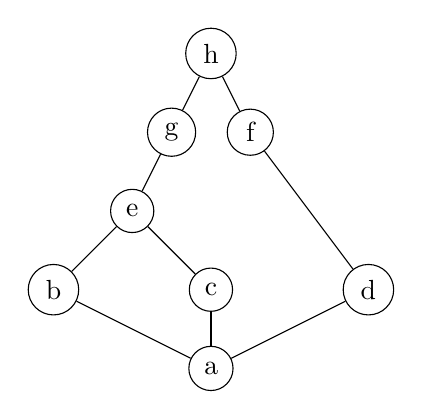
\begin{tikzpicture}[>=stealth, node distance=2cm]
    \node[draw, circle] (a) at (0,0) {a};
    \node[draw, circle] (b) at (-2,1) {b};
    \node[draw, circle] (c) at (0,1) {c};
    \node[draw, circle] (d) at (2,1) {d};
    \node[draw, circle] (e) at (-1,2) {e};
    \node[draw, circle] (f) at (0.5,3) {f};
    \node[draw, circle] (g) at (-0.5,3) {g};
    \node[draw, circle] (h) at (0,4) {h};

    \draw (a) -- (b);
    \draw (a) -- (c);
    \draw (a) -- (d);
    \draw (b) -- (e);
    \draw (c) -- (e);
    \draw (d) -- (f);
    \draw (e) -- (g);
    \draw (f) -- (h);
    \draw (g) -- (h);
\end{tikzpicture}
\end{figure}
\subsection{T29}
(a) $\{a\}, \{b\}, \{c\}$\\
(b) $2, 3, 5$
\subsection{T32}
(a) 原子:$001, 010, 100$。其他元素的原子表示:$110 = 100 \lor 010 \quad 101 = 100 \lor 001 \quad 
011 = 010 \lor 001 \quad 111 = 100 \lor 010 \lor 001$。\\
(b) 原子:$2, 3, 7$。其他元素的原子表示:$6 = 2 \lor 3 \quad 21 = 3 \lor 7 \quad 42 = 2 \lor 3 \lor 7$。\\
(c) 原子:$
\begin{bmatrix}
    1 & 0\\
    0 & 0
\end{bmatrix},
\begin{bmatrix}
    0 & 1\\
    0 & 0
\end{bmatrix},
\begin{bmatrix}
    0 & 0\\
    1 & 0
\end{bmatrix},
\begin{bmatrix}
    0 & 0\\
    0 & 1
\end{bmatrix}$.\\
其他元素的原子表示:
$$
\begin{bmatrix}
    1 & 1\\
    0 & 0
\end{bmatrix}
=
\begin{bmatrix}
    1 & 0\\
    0 & 0
\end{bmatrix}
\lor
\begin{bmatrix}
    0 & 1\\
    0 & 0
\end{bmatrix}
\quad 
\begin{bmatrix}
    1 & 0\\
    1 & 0
\end{bmatrix}
=
\begin{bmatrix}
    1 & 0\\
    0 & 0
\end{bmatrix}
\lor
\begin{bmatrix}
    0 & 0\\
    1 & 0
\end{bmatrix}
$$
$$
\begin{bmatrix}
    1 & 0\\
    0 & 1
\end{bmatrix}
=
\begin{bmatrix}
    1 & 0\\
    0 & 0
\end{bmatrix}
\lor
\begin{bmatrix}
    0 & 0\\
    0 & 1
\end{bmatrix}
\quad 
\begin{bmatrix}
    0 & 1\\
    1 & 0
\end{bmatrix}
=
\begin{bmatrix}
    0 & 1\\
    0 & 0
\end{bmatrix}
\lor
\begin{bmatrix}
    0 & 0\\
    1 & 0
\end{bmatrix}
$$
$$
\begin{bmatrix}
    0 & 1\\
    0 & 1
\end{bmatrix}
=
\begin{bmatrix}
    0 & 1\\
    0 & 0
\end{bmatrix}
\lor
\begin{bmatrix}
    0 & 0\\
    0 & 1
\end{bmatrix}
\quad 
\begin{bmatrix}
    0 & 0\\
    1 & 1
\end{bmatrix}
=
\begin{bmatrix}
    0 & 0\\
    1 & 0
\end{bmatrix}
\lor
\begin{bmatrix}
    0 & 0\\
    0 & 1
\end{bmatrix}
$$
$$
\begin{bmatrix}
    1 & 1\\
    1 & 0
\end{bmatrix}
=
\begin{bmatrix}
    1 & 0\\
    0 & 0
\end{bmatrix}
\lor
\begin{bmatrix}
    0 & 1\\
    0 & 0
\end{bmatrix}
\lor
\begin{bmatrix}
    0 & 0\\
    1 & 0
\end{bmatrix}
\quad 
\begin{bmatrix}
    1 & 1\\
    0 & 1
\end{bmatrix}
=
\begin{bmatrix}
    1 & 0\\
    0 & 0
\end{bmatrix}
\lor
\begin{bmatrix}
    0 & 1\\
    0 & 0
\end{bmatrix}
\lor
\begin{bmatrix}
    0 & 0\\
    0 & 1
\end{bmatrix}
$$
$$
\begin{bmatrix}
    1 & 0\\
    1 & 1
\end{bmatrix}
=
\begin{bmatrix}
    1 & 0\\
    0 & 0
\end{bmatrix}
\lor
\begin{bmatrix}
    0 & 0\\
    1 & 0
\end{bmatrix}
\lor
\begin{bmatrix}
    0 & 0\\
    0 & 1
\end{bmatrix}
\quad 
\begin{bmatrix}
    0 & 1\\
    1 & 1
\end{bmatrix}
=
\begin{bmatrix}
    0 & 1\\
    0 & 0
\end{bmatrix}
\lor
\begin{bmatrix}
    0 & 0\\
    1 & 0
\end{bmatrix}
\lor
\begin{bmatrix}
    0 & 0\\
    0 & 1
\end{bmatrix}
$$
$$
\begin{bmatrix}
    1 & 1\\
    1 & 1
\end{bmatrix}
=
\begin{bmatrix}
    1 & 0\\
    0 & 0
\end{bmatrix}
\lor
\begin{bmatrix}
    0 & 1\\
    0 & 0
\end{bmatrix}
\lor
\begin{bmatrix}
    0 & 0\\
    1 & 0
\end{bmatrix}
\lor
\begin{bmatrix}
    0 & 0\\
    0 & 1
\end{bmatrix}
$$
\section{6.5}
\subsection{T11}
\begin{align*}
    (x \land y' \land z) \lor (x \land y \land z) &= (y' \land (x \land z)) \lor (y \land (x \land z))\\
    &= (y \lor y') \land (x \land z)\\
    &= 1 \land (x \land z)\\
    &= x \land z
\end{align*}
\subsection{T12}
\begin{align*}
    (z \lor (y \land (x \lor x'))) \lor (y \land z)' &= (z \lor (y \land 1)) \land (y \land z')'\\
    &= (z \lor y) \land (y' \lor z)\\
    &= z \land (y \lor y')\\
    &= z
\end{align*}
\subsection{T13}
\begin{align*}
    (y \land z) \lor x' \lor (w \land w') \lor (y \land z') &= x' \lor 0 \lor (y \land z') \lor (y \land z)\\
    &= x' \lor (y \land (z \lor z'))\\
    &= x' \lor y
\end{align*}
\subsection{T14}
$(x' \land y' \land z' \land w) \lor (x' \land z' \land w' \land y') \lor 
(w' \land x' \land y \land z') \lor (w \land x' \land y \land z)
= (x' \land y' \land z') \lor (x' \land y \land z') = (x' \land z')$
\subsection{T18}
$(x \lor (y \land z))' \lor z'$
\subsection{T19}
$((x \land y) \lor (y \land z))'$
\subsection{T20}
$(x' \land x)' \lor ((y \land w') \lor ((y \land w) \lor z'))$
\subsection{T21}
\begin{align*}
    (x \lor (y \land z))' \lor z' &= (x' \land (y \land z)') \lor z'\\
    &= (x' \land (y' \lor z')) \lor z'\\
    &= (x' \land y') \lor (x' \land z') \lor z'\\
    &= (x' \land y') \lor z'\\
    &= (x \lor y)' \lor z'\\
    &= ((x \lor y) \land z)' 
\end{align*}
\begin{figure}[h]
    \centering
    \includegraphics[width=0.75\textwidth]{T21.png}
\end{figure}
\subsection{T22}
$((x \land y) \lor (y \land z))' = (y \land (x \lor z))'$
\begin{figure}[h]
    \centering
    \includegraphics[width=0.75\textwidth]{T22.png}
  \end{figure}
\subsection{T23}
\begin{align*}
    (x' \land x)' \lor ((y \land w') \lor ((y \land w) \lor z')) &= 1 \lor ((y \land w') \lor (y \land w) \lor z')\\
    &= y \lor z'
\end{align*}
\begin{figure}[h]
    \centering
    \includegraphics[width=0.75\textwidth]{T23.png}
\end{figure}
\section{6.6}
\subsection{T8}
\begin{figure}[h]
    \centering
    \includegraphics[width=0.75\textwidth]{T8.png}
\end{figure}
\subsection{T12}
$(y' \land z) \lor (x' \land z') \lor (x \land y \land z')$
\subsection{T14}
$(x' \land y') \lor (x' \land y) \lor (y \land z) = x' \lor (y \land z)$
\subsection{T16}
$(x' \land z') \lor (x' \land w' \land z) \lor (x \land y' \land w')$
\subsection{T24}
\begin{figure}[h]
    \centering
    \includegraphics[width=0.75\textwidth]{T8.png}
\end{figure}
由下图可得:$f = (x' \land y' \land w) \lor (x \land y' \land w') \lor (x' \land y \land w' \land z') \lor (x \land y \land w \land z')$
\subsection{T25}
(a) $(0, 0) \rightarrow x' \land y' \quad (0, 1) \rightarrow x' \land y \quad (1, 0) \rightarrow x \land y'$\\
(b) 设元素$s_1, s_2$分别表示为$x_1x_i$,\quad$x_1(x_i)'$因此$s_1 \lor s_2 = (x_1 \land x_i) \lor (x_1 \land x_i') = x_1 \land (x_i \lor x_i') = x_1$.
因此不需要变量$x_i$。
\subsection{T26}
(a) $x' \lor y'$\\
(b) 
$$
\begin{array}{|c|c|c|c|}
    x & y & x' \lor y' & f\\
    \hline
    0 & 0 & 1 & 1\\
    0 & 1 & 1 & 1\\
    1 & 0 & 1 & 1\\
    1 & 1 & 0 & 0
\end{array}
$$
因此$f$是由(a)中的$x' \lor y'$产生的。
\end{document}